\section{Plugin for the RAVEN Code}
\label{sec:RavenPlugin}

The deterministic model can be repeatedly solved by changing the input values (i.e.,
\xmlNode{available\_capitals} [$b_{kt}$] and \xmlNode{net\_present\_values} [$a_{ij}$]).
This will allow for what-if sensitivity analysis to identify the
crucial drivers behind the optimal project selection decision. Monte Carlo simulation permits a
powerful variant of this approach in which we model $a_{ij}$ and $b_{kt}$ as random
variables, sample from their distributions, and perform a form of uncertainty quantification
in terms of the resulting distributions governing the binary decisions selected, $x_{ij}$, and
the overall NPV of the selected portfolio.

Example RAVEN input \xmlNode{ExternalModel} XML:
\begin{lstlisting}[style=XML]
<Models>
  <ExternalModel name="singleKnapsack" subType="LOGOS.CapitalInvestmentModel">
    <variables>available_capitals,i1,i2,i3,i4,i5,i6,i7,i8,i9,i10,
      MaxNPV</variables>
    <ModelData>
      <Sets>
        <investments>
          i1,i2,i3,i4,i5,i6,i7,i8,i9,i10
        </investments>
      </Sets>
      <Parameters>
        <net_present_values index="investments">
          18,20,17,19,25,21,27,23,25,24
        </net_present_values>
        <costs index="investments">
          1,3,7,4,8,9,6,10,2,5
        </costs>
        <available_capitals>
          15
        </available_capitals>
      </Parameters>
      <Settings>
        <solver>glpk</solver>
        <sense>maximize</sense>
      </Settings>
    </ModelData>
  </ExternalModel>
</Models>
\end{lstlisting}

As the name suggests, an external model is an entity that is embedded in the RAVEN
code at run time. This object allows the user to import the LOGOS module that will
be treated as a predefined internal RAVEN object. In other words, the
\textbf{External Model} will be treated by RAVEN as a normal external model.
Check the RAVEN user manual for a more detailed description.
\nb The value for attribute \xmlAttr{subType} should always be \xmlString{LOGOS.CapitalInvestmentModel}.

\xmlNode{variables} specifies a list of variable names that need to match
variables used/defined in the LOGOS model. In the above example, the variable
\xmlString{available\_capitals} is sampled by RAVEN, and its value is used
by LOGOS instead of using the default values specified by \xmlNode{ModelData}.
The decision variables \xmlString{i1,i2,i3,i4,i5,i6,i7,i8,i9,i10} and the
objective variable \xmlString{MaxNPV} are collected from the output of the LOGOS model,
and can be stored in the RAVEN data objects.
The XML node \xmlNode{ModelData} is used to specify the LOGOS optimization problem, which
should be consistent with the LOGOS input XML file.

\subsection{Test Automation}
Automated regression testing is a development methodology generally used
to verify the correctness and performance of software after each modification.
This methodology is integrated directly into GitHub and GitLab for RAVEN and
RAVEN-supported plugins. In this case, testing is performed automatically as part of the
continuous integration system (CIS) process whenever a user commits a change to the
repository. Tests of changes across multiple platforms are executed with each pull
request. Results from each test execution are maintained in an approved records
repository in the CIS database, along with results from the timing executions.

\subsection{Testing System Prerequisites}
The module test system consists of scripts written in Bash shell language
and Python. It may be used on any platform supported by RAVEN (i.e.
Linux, Mac, and Windows). The following conditions must be satisfied for the
module test system to function properly:
\begin{itemize}
  \item RAVEN should be installed and updated. This is because RAVEN is used to
  run the module tests;
  \item The system running the tests must be configured with the software prerequisites
  necessary to build and run RAVEN. These include a Python interpreter, Python
  libraries (h5py, matplotlib, numpy, scipy, and scikit-learn), and development
  tools (C++ compiler, Miniconda package manager for Python, and Git source code control);
  \item RAVEN must be built with the appropriate compiler before it can be used to
  run the tests;
  \item The LOGOS submodule must be initialized and fully updated. Additional prerequisites
  include PYOMO, glpk, and coincbc;
\end{itemize}

\subsection{Test Location and Definition}
LOGOS is a RAVEN-supported plugins and managed by Git. RAVEN plugins afford
an option to associate a workflow or a set of RAVEN external models to RAVEN
without having them included in the RAVEN main repository. The benefits include
modularity, access restriction, and regression testing for compatibility with RAVEN
as it continues to grow. In this case, we are able to treat this repository as
separate, yet still be able to use one from within the other. The main structure
of the LOGOS repository is shown in Figure~\ref{fig:Logos}. The folder \textit{tests} contains the input of
the tests, in addition to the corresponding output (in the gold folder) used for
assurance that the behavior of the code is not changed for new modifications. These
tests can also be collected in subfolders based on their characteristics.

\begin{figure}
    \centering
    \centerline{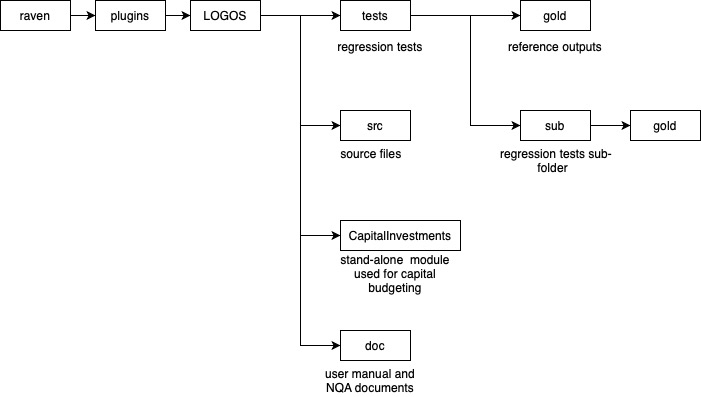
\includegraphics[scale=0.5]{LogosRepo.jpg}}
    \caption{Folder tree of the Logos repository.}
    \label{fig:Logos}
\end{figure}

The RAVEN repository contains a complete testing system for providing regression
testing for itself and its plugins. The LOGOS module tests are defined in the
same manner as for RAVEN. A single test consists of a RAVEN input file
along with associated data needed to perform that run. This can include input data,
external models, and Python files. These may be placed in the \textit{tests} directory
or a related subdirectories. Each directory that contains tests to be run by
the framework must contain a test specification file named “tests”. The syntax of
these files is defined by the RAVEN test framework, which controls how each test
is run and sets the criteria used to determine whether it passed or not. An example
of a test specification file is presented here:
\begin{lstlisting}[language=python]
[Tests]
  [./skp_optimization]
    type = 'RavenFramework'
    input = 'test_skp.xml'
    UnorderedCsv = 'skp/test_skp.csv'
  [../]
[]
\end{lstlisting}
In the above example, one test, named ``skp\_optimization'', is defined using the RAVEN
test module (defined in the test file as “type = `RavenFramework'”). Comparison
criteria are also defined in the “tests” file. In most cases, one or more output
files generated by running the specified input file with RAVEN are compared
against a gold standard provided by the developer and stored in the repository.
Typically, comparisons are performed on numeric values contained in
CSV files up to a defined tolerance. When these file comparisons are specified
by the test developer, reference files must have the same name and be placed
in the gold subdirectory below that containing the “tests” file.

\subsection{Running the Tests}
The integrated tests can be run separately, as indicated by following this pathway:
\begin{lstlisting}[language=bash]
path/to/raven/raven_framework path/to/LOGOS/tests/TestName
\end{lstlisting}

\subsection{Continuous Integration System (CIVET)}
CIVET, developed at INL, is used for continuous integration, verification,
enhancement, and testing of RAVEN and LOGOS. Each time a developer
proposes modification of the contents of the LOGOS repository, CIVET will cause
the automated tests to be run on the modified version. These tests must all pass
before a proposed change can become part of the official repository. In this way,
the LOGOS project is protected from the accidental introduction of flaws into
software that required such a significant investment of resources to develop.
